\documentclass[letterpaper,twocolumn,10pt]{sig-alternate-10pt}

%%%%%%%%%%%% LIST OF PACKAGES
\usepackage{epsfig,endnotes}
\usepackage[usenames,dvipsnames]{color}
\usepackage[english,plain]{fancyref}
\usepackage{times}
\usepackage{rotating}
\usepackage{subfig}
\usepackage{multirow}
\usepackage{amsfonts,xspace}
\usepackage{url}
\usepackage{graphicx}


%%%%%%%%%% LIST OF COMMANDS
\newcommand{\ie}{{\it i.e.}\xspace}
\newcommand{\eg}{{\it e.g.}\xspace}
\newcommand{\etc}{{\it etc.}}
\newcommand{\etal}{\emph{et~al.}}
\newcommand{\useragent}{{\it User-Agent}\xspace}
\newcommand{\httphost}{{\it Host}\xspace}
\newcommand{\httpget}{{\it HTTP GET}\xspace}
\newcommand{\wifi}{{Wi-Fi}\xspace}
\newcommand{\sslservername}{{\it Server-Name}\xspace}
\newcommand{\eat}[1]{}
%% tbd
\newcommand{\tbd}[1]{[{\color{red}{\bf{TBD: #1}}}]}
\newcommand{\artbd}[1]{[{\color{blue}{\bf{AR:TBD: #1}}}]}
\newcommand{\dtbd}[1]{[{\color{blue}{\bf{Dave:TBD: #1}}}]}
% platform
\newcommand{\meddle}{{\emph{Meddle}}\xspace}
\newcommand{\meddlebox}{{\emph{meddlebox}}\xspace}

\newcommand{\mypara}[1]{\medskip\noindent{\bf {#1}:}~}
\newcommand{\chk}{$\checkmark$}
\newcommand{\dsh}{{\bf --}}
\newcommand{\til}{{\bf\large \textasciitilde}}
\newcommand{\drc}[1]{[{\color{blue}{Dave: #1}}]}
%\newcommand{\tbd}[1]{}
\newcommand{\tbdv}[1]{{\color{blue}{!\bf{#1}$_{verify}$}!}}
\newcommand{\platname}{{\emph{Meddle}}\xspace}
\newcommand{\platnameT}{{Meddle}\xspace}
\newcommand{\dsum}{\displaystyle\sum}
\newcounter{packednmbr}
\newcommand{\iphone}{iPhone\xspace}
\newcommand{\postfigspace}{-1em}
\newcommand{\figcapspace}{0em}
\newcommand{\mobWild}{{\emph{mobWild}}\xspace}


\newenvironment{packedenumerate}{\begin{list}{\thepackednmbr.}{\usecounter{packednmbr}\setlength{\itemsep}{0.2pt}\addtolength{\labelwidth}{-4pt}\setlength{\leftmargin}{\labelwidth}\setlength{\listparindent}{\parindent}\setlength{\parsep}{1pt}\setlength{\topsep}{0pt}}}{\end{list}}
\newenvironment{packeditemize}{\begin{list}{$\bullet$}{\setlength{\itemsep}{0.2pt}\addtolength{\labelwidth}{-4pt}\setlength{\leftmargin}{\labelwidth}\setlength{\listparindent}{\parindent}\setlength{\parsep}{1pt}\setlength{\topsep}{0pt}}}{\end{list}}


\begin{document}

\date{}

\title{{\Large \bf Using the Middle to Meddle with Mobile}} 
%\\
%{\large A Practical Approach to Improving Transparency and Control for Mobile Networking}}


\author{}
%\large Ashwin Rao${^a}$, Amy Tang${^b}$, Shen Wang${^c}$, Nick Martindell${^c}$, Justine Sherry${^b}$, Arnaud Legout${^a}$, \\
%\large Walid Dabbous${^a}$, Arvind Krishnamurthy${^c}$, and David Choffnes${^d}$\\ 
%\large $^{a}$INRIA $^{b}$University of California, Berkeley \\
%\large $^{c}$University of Washington $^{d}$Northeastern University
%} 

\maketitle

% Use the following at camera-ready time to suppress page numbers.
% Comment it out when you first submit the paper for review.
%\thispagestyle{empty}

\subsection*{Abstract}
{\it Researchers and mobile users have little visibility into the network 
traffic generated by  mobile devices and have poor control over 
how, when, and where that traffic is sent and handled. 
This paper presents Meddle, a platform that  leverages 
VPNs and software middleboxes to improve transparency and control 
for Internet traffic from mobile systems. Meddle provides a practical way to 
interpose on all of a device's Internet traffic, while providing clear incentives, privacy guarantees, 
and ease of deployment to end users. We discuss 
the design and implementation of our system, and evaluate its effectiveness with  
measurements from an IRB-approved user measurement study. We demonstrate the 
potential of this platform using case studies of application built atop Meddle; namely,
controlling privacy leaks, detecting ISP interference with 
Internet traffic, and blocking malware.
}






%%% Local Variables: 
%%% mode: latex
%%% TeX-master: "meddle-main"
%%% End: 


%Note one sentence in one text line.
\section{Introduction}
\label{sec:introduction}

%Mobile systems consist of walled gardens inside gated communities, i.e., locked-down operating systems running on devices that interact over a closed and opaque mobile network. 

Our contributions are as follows
\begin{itemize}
\item We posit that VPNs can be used build a practical platform to monitor mobile Internet traffic regardless of the mobile operating system, device type, access technologies, and service provider.
\item We present \platname, a practical platform for comprehensive monitoring of mobile Internet traffic. 
\platname builds on existing functionality provided by Mobile OSes to manage VPN tunnels. 
\item We use \platname to compare the behavior of popular mobile applications over Android and iOS. We observe \tbd{values come here}. We also compare the behavior of these application over Wifi and 3G. 
\item \tbd{Results based on Amy work}.
\item \tbd{Results from an on going IRB based study of 30 users. We use these results to compare our observations from exisiting studies. The key take home is that these measurements were did not require custom OSes, ISP support, or support from marketplaces, warranty voiding of devices.}
\end{itemize}

\tbd{Things to highlight in Intro\\
Tools\\
Techniques\\
Methodology\\
Insights}







%Note one sentence in one text line.
\section{VPN Based Mobile Measurement Platform} 
\label{sec:platform} 
In this section, we enumerate the goals of a mobile measurement platform, show how VPNs can be used to achieve the described goals, and finally present empirical results that demonstrate the feasibility of \platname, a VPN based platform for mobile network traffic measurement.

\subsection{Goals}  
\label{sec:goals} 
The primary goal for our platform is to provide comprehensive visibility into mobile networking traffic. 
To meet this goal, we further identify the following sub-goals that address limitations of the existing platforms discussed in \fref{sec:motivation}.
\begin{packedenumerate}
\item \emph{Portable.} We want our solution to work regardless of operating system, access technology, and service provider. 
\item \emph{Pervasive.} For maximum transparency, our system should provide seamless visibility into all network traffic generated by devices. 
This means continuous monitoring over time and as users move with their 
\item \emph{Passive} For comprehensive and independent of user triggers we want our solution to passively perform measurements. 
\item \emph{Deployable.} Our solution should be easy to use, immediately deployable and incur reasonable costs (or none at all) for users.
Furthermore, it should not incur the cost of warranty-voiding the device and by relying on techniques such as rooting a phone.
\end{packedenumerate}    

\subsection{Description}
\label{sec:description}

We believe that VPNs can be used to setup a portable, pervasive, and deployable measurement platform for mobile device. 
Our motivation was the use of VPNs by executives ``on the move'' to securely connect to corporate servers with their mobile device. 
The use of VPNs by corporate clients gave us hints towards considering VPNs as portable and deployable platform.
Further investigation showed us that Mobile OSes expose features that can make them pervasive.  


\subsubsection{Mobile Devices}

All iOS devices (version 3.0 and above) come with a feature called ``VPN On-Demand''. 
\emph{VPN On-Demand} forces the iOS device to use VPN tunnels when connecting to a specified set of domains. 
We use this feature to enforce our iOS devices to use a VPN tunnel to connect to the Internet.

Android version 4.0 and above comes with native VPN support. 
Unlike iOS, Android does not offer an equivalent of \emph{VPN On-Demand}; however, Android provides an API that allows an user space app to manage VPN connections. 
We modify the open source StrongSwan VPN client~\cite{strongswanclient} to ensure that the VPN reconnects each time the preferred network changes (\eg, when a device switches from cellular to \wifi). 
As of Android 4.2, Android supports ``Always On'' VPN connections that uses VPNs to tunnel all the data traffic. 
\tbd{Text on Issues with Always ON}.

\subsubsection{VPN Server}
Strongswan, Openswan, and OpenVPN are some of the popular VPN daemons that can be used to manage VPN tunnels. 
We use Strongswan because it is open source and, to the best of our knowledge, it is the only open source solution that can use the IPsec services of the Linux kernel without any kernel modifications. 
IPsec is important because the \emph{VPN On-Demand} feature of iOS is supported only for VPN tunnels that use IPsec. 
Strongswan is supported on vanilla Linux operating systems which ensures that VPN tunnels can be managed using \emph{off-the-shelf} software and hardware.

In summary, the active use of VPNs to access corporate networks regardless of the ISP, access technology motivated us to consider VPNs. 
Mobile devices can connect to open source VPN implementation that can run on off-the-shelf servers. 
Our platform relies on VPNs to tunnel and capture the mobile data traffic. 
We use the open source Strongswan daemon to manage VPN tunnels. 
We use tcpdump to capture the packets on the server that runs Strongswan. 
Our servers have been deployed at the University of Washington and Inria and the mobile devices belong to users participating in an IRB-approved study. 

\tbd{How we capture and why this is important to label flows to access
technology and ISP?New instance of tcp dump for each flow. Each time a
tunnel is created separate instance of tcpdump used -- required to isolate
flows. We log the IP address from which tunnel is created. We use this IP
to get the details of the ISP. We then look up the ISP and label the
connection to be wifi or celluar. Pros and cons of this approach.}

\eat{
\begin{figure}
\includegraphics[width=0.75\columnwidth]{figures/meddle-servers.pdf}
\caption{\tbd{I am not sure if we need this figure}}
\label{fig:description}
\end{figure}
}

\subsection{Feasibility}

We now show that a VPN based platform is portable, pervasive, deployable, and incurs a small overhead in terms of latency, power, and bandwidth. 

\subsubsection{Portable, Pervasive, Passive, and Deployable} 
% device, access technology, and service provider. 
Android, BlackBerry, Bada, and iOS all support VPNs natively, representing more than 86\% of the mobile device market\cite{gartner-phone-share}. 
These devices support VPN tunnels over Wi-Fi and the cellular interface.
Furthermore, to satisfy their corporate clients, very few ISPs are known to block VPN traffic to flow through their networks.  

% devices connect seamlessly without periodic action.
We use the ``VPN On-Demand'' feature provided by iOS to ensure that our system is pervasive. 
Android provides an API that allows user space apps to manage VPN connections. 
We modify the open source StrongSwan VPN client~\cite{strongswanclient} to ensure that the VPN reconnects each time the preferred network changes (\eg, when a device switches from cellular to \wifi). 
As of Android 4.2, Android supports ``Always On'' VPN connections that uses VPNs to tunnel all the data traffic. 
\tbd{Text on Issues with Always ON}.

Manually configuring a VPN generally requires filling out five fields on an Android phone, and the VPN configuration can be distributed using a single file on iOS.
These configurations are primarily required to drive the key exchange algorithms that establish the VPN tunnels. 
This simplicity is important because it can facilitate realistic measurement studies with end users.  

In summary, native VPN support along with a set of features exposed to by mobile OSes to manage VPNs offer a solid foundation to build a portable, pervasive, passive, and deployable platform for mobile measurements.

\subsubsection{Latency Overheads}
Number of round trip times to establish the connection. 
\tbd{Text from results from Adrian and Sam}

\subsubsection{Power Overheads}
\tbd{TODO if needed}

\subsubsection{Bandwidth Overheads} 

Number of packets to establish the connection 

IPSec encapsulation slightly inflates packet sizes, in addition to preventing carrier middleboxes from applying their own compression. 
We measured the overhead of the tunnel in terms of data overhead from IPsec headers and keep-alive messages, finding that it ranges from \tbd{range}\%.

For our measurements, we capture the encrypted packets exchanged by our servers and the clients that use \platname. 
We performed the packet capture for \tbd{Number} days during which \tbd{number} devices tunneled their traffic via our  servers. 
During this time interval we also capture the packets that were encapsulated in the IPsec packets. 
We use these samples to compute the increase in the amount of bytes transferred due to encapsulation and the keep-alive messages. 
During the 14 day period we observe that the median of the increase to be \tbd{number}\%, with a maximum increase of \tbd{number}\%

\tbd{In Summary, ...}


\section{Methodology and Dataset}
\label{sec:Methodology}

We used \platname to characterize mobile Internet traffic, and detail the impact of access technology and operating systems on application behavior. 

Our analysis methodology included controlled experiments to detail the behavior of specific applications and OS services, and a 7-month long IRB approved measurement study to characterize mobile Internet traffic in the \emph{in the wild} . 

\subsection{Controlled Experiments}

For our controlled experiments, we ran the latest versions of Android (Ice Cream Sandwich 4.0, and Jelly-bean 4.2) and iOS 6 respectively on our Android and iOS devices. 
We analyze the behavior of OS services and the default applications by first performing a factory reset on these devices, and installing the \platname credentials on this device.
We then test Android and iOS applications by installing the application, interacting with the application for a few minutes, and finally uninstalling the  application. 
During our controlled experiment we use SSL-Bumping to study the behavior of SSL traffic from these applications. 

Our first experiment included manual testing of the top 100 most popular free Android apps from the \emph{Google Play} store and \tbd{} iOS applications from the iOS App store.
For this experiment we first manually installed each application by hand, enter user credentials for accounts like Facebook and Twitter, and toy with the app for \tbd{} minutes. 
In addition to this manual setup, we used an automatic test-click generator to further toy with the Android applications for \tbd{} actions. 
We did not perform this automation step while testing the the iOS applications.
We then uninstall the application and reset the device to test the next application. 

For our second experiment we performed fully-automated tests on 1003 Android applications from a free, third-party Android market.
We perform this test because Android devices can install \emph{Third-party applications} that are not available on the \emph{Google Play} store.
A consequence of this freedom is that numerous third-party app markets are available on the web whose applications have not received research attention.
Our automation used the adb Android command shell to install each app, enable \platname, and start the app.
The system then used Monkey, an adb stress tool, to perform a series of 10,000 actions. 
These actions included random swipes, touches, and text entries.
We then used adb to uninstall the application and reboot the device to forcibly end any lingering connections.

The results of the controlled experiments can be found in \fref{sec:manual-testing}.

\subsection{In The Wild Measurements}

Along with controlled experiments we also conducted a measurement study to characterize the mobile Internet in the wild.
We now present the description of the dataset and the methodology we used to classify the traffic in this dataset.

\subsubsection{Dataset Description}

For this study, we deployed two \platname servers, one in USA and one in France, to proxy Internet traffic from 26 devices, 10 iPhones, 4 iPads, 1 iPodTouch, and 11 Android phones.
The Android devices in this dataset include the Nexus, Sony, Samsung, and Gsmart brands while the iPhones include one iPhone~3gs, five iPhone~5, and five iPhone~4S.
These devices belonged to 21 users, volunteers for our IRB approved study.
%To protect the identity of the users and their data, we used public key cryptography to encrypt the \emph{pcap} files that log the data traffic flowing through our \platname servers. 
This dataset, called \mobWild, consists of 218 days of data that flowed through our \platname servers; the number days for each user varies from 5 to 215 with a median of 35 days.
We would like to point out that though we performed SSL-Bumping during our controlled experiments, we did not perform SSL-Bumping for the traffic in this dataset.

\subsubsection{Ethical Issues}

Capturing all of a subject's Internet traffic raises significant
privacy concerns. Our IRB-approved study entails informed consent from
subjects who are interviewed in lab, where the risks and benefits of
our study are clearly explained. Subjects are incentivized to use the
VPN though a lottery for Amazon.com gift certificates. All data from
tcpdump is encrypted before touching persistent storage; the private
key is maintained on separate secure severs and only approved
researchers can access it. Users may delete their data and/or disable
monitoring at any time. For privacy reasons, we cannot make this data
publicly available.


\subsubsection{Identification of Access Technology}

A mobile devices can tunnel the traffic through our \platname servers using either \wifi or cellular networks. 
We estimate the access technology with the description of the AS through which the mobile client connects to our \platname server. 
We get this AS description by performing a \emph{WHOIS} lookup on the IP address used by the mobile client to tunnel Internet traffic. 
For our analysis, we use the WHOIS databases available at \emph{whois.cmyru.com} and \emph{utrace.de}.
We use the information from these \emph{WHOIS} databases to manually classify the ASes to be either cellular or \wifi.
Our dataset consists of data traffic from 54 distinct ASes, of which we classify 9 to be belong to cellular networks.
The devices connected to our system from at most two cellular ASes.
In contrast, a median of 4 \wifi ASes were observed per device and for one device we observed traffic from 25 different \wifi ASes that are spread across 5 countries. 


\subsubsection{Traffic Summary}

\begin{table}
\begin{small}
\begin{center}
\begin{tabular}{|p{0.15\columnwidth}|p{0.12\columnwidth}|r|r|r|r|}
\hline
\multirow{2}{*}{\bf IP Protocol} & \multirow{2}{*}{\bf Service} & \multicolumn{2}{|c|}{\bf Android} & \multicolumn{2}{|c|}{\bf iOS} \tabularnewline
\cline{3-6}
           &           &  \textbf{Cell.}  &  \textbf{\wifi}  &  \textbf{Cell.}  &  \textbf{\wifi}  \tabularnewline
\hline
\multirow{3}{*}{TCP}
       &  HTTP  & 35.386 & 68.686 & 52.109 & 75.506 \tabularnewline
\cline{2-6}
       &  SSL   & 61.135 & 27.366 & 46.765 & 18.777 \tabularnewline
\cline{2-6}
       &  other & 2.346  & 3.290  & 0.256  & 1.818 \tabularnewline
\hline
\multirow{2}{*}{UDP}
       &  DNS   & 0.682  & 0.496  & 0.545  & 0.305  \tabularnewline
\cline{2-6}
       &  other & 0.316  & 0.098  & 0.286  & 3.583  \tabularnewline
\hline
 Other &  -     & 0.135  & 0.064 & 0.039  & 0.011  \tabularnewline
\hline
\multicolumn{2}{|c|}{\emph{total}} & 100.00 & 100.00 & 100.00 & 100.00 \tabularnewline
\hline
\end{tabular}
\end{center}
\end{small}
\caption{Traffic volume (in percentage) of popular protocols and services on Android and iOS devices over cellular and \wifi.
\emph{TCP flows are responsible for more than 90\% of traffic volume. Traffic share of SSL over cellular networks is more than twice the traffic share of SSL over \wifi.}} 
\label{tab:summaryIOSAndroidTraffic}
\end{table}

We used Bro~\cite{bro} to analyze the traffic the passed through our \platname servers.
In \fref{tab:summaryIOSAndroidTraffic} we summarize \mobWild based on the classification performed using Bro~\cite{bro}.
Bro classifies IP flows using the protocol field in the IP header.
We use this classification to label flows as either TCP, UDP, or \emph{other}; flows that are neither TCP nor UDP are classified as \emph{other}. 
Bro further uses the well defined port numbers to identify the services that use TCP.
We use this classification to label flows as either HTTP, SSL (which includes HTTPS, IMAP, etc.) or \emph{other} flows; TCP flows that are not classified as either HTTP or SSL are classified as \emph{other}.
In \fref{tab:summaryIOSAndroidTraffic}, we observe that more than 90\% of the traffic in our dataset is either HTTP or SSL. 
We also observe that the share of HTTP volume over \wifi and cellular are significantly different. 
As detailed in \fref{sec:.}, this difference is primarily due to the use of \wifi to transfer media content.
We also observe the share of SSL traffic over cellular networks is considerably larger compared to \wifi networks.
This increase is a result of the reduced share of media traffic and the use of email and for social networking applications that rely on SSL.
We detail the HTTP and SSL traffic from iOS and Android devices in \fref{sec:}

We focus our application classification on TCP because TCP is responsible for than 90\% of the traffic volume in our dataset (see~\fref{tab:summaryIOSAndroidTraffic}).
Furthermore more than 95\% of the TCP traffic is due to SSL and HTTP.
We therefore focus our attention on HTTP and SSL traffic. 

\subsubsection{Classification of HTTP Traffic}

The HTTP headers for HTTP Request, HTTP Response, and HTTP Entity contain a wealth of information including \useragent, \emph{Referrer}, \emph{Content-Type}, and \emph{Content-Encoding} that can be used to classify HTTP traffic~\cite{rfc:http}.
Recent studies on mobile traffic classification have relied heavily on the \useragent field to classify mobile HTTP traffic~\cite{qian:webcache, maier:mobtraffic, xu:appusage}.
We quantify the usefulness of the \useragent field and show how other fields such as \httphost are essential to characterize mobile HTTP traffic. 

Webservices are known to use the \useragent field to distinguish flows from their mobile applications from the flows originating from Web-browsers.
We observe that more than 98\% of HTTP traffic from Android and iOS devices in the \mobWild dataset have a valid \useragent string; we observe a total of 1435 unique \useragent strings across Android and iOS devices. 
In these \useragent strings we observe that along with the application identifier, the \useragent strings also contain details of the OS, manufacturer, display resolutions, carrier, and other information such as versions and compatibility with other browser engines. 
We use regular expression to extract the tokens containing the application information and we then cluster these tokens using edit distance between individual tokens and number of matching tokens. 
We plan to release this code along with \platname package.
At the end of this process we were able to identify 361 unique application signatures.
We use the extracted application signature to label the HTTP traffic that flows through \platname.

\begin{figure}
\includegraphics[width=\columnwidth]{plots/appusage_someappsig_traffic.pdf}
\caption{HTTP traffic with a \useragent field containing an identifier of an application (other than Web-browser) or an OS service. 
\emph{A smaller share of Android HTTP traffic can be classified using User-Agents because Android applications are not limited to underlying OS media services such as AppleCoreMedia.}}
\label{fig:http-classification-app-user-agent}
\end{figure}

In \fref{fig:http-classification-app-user-agent} we plot the fraction of HTTP traffic for we were able to identify an application signature; the devices are ordered according to the operating system, and for each operating system we further order the devices according to the total traffic from the device that flowed through \platname. 
We observe that a significantly larger fraction of traffic from iOS device can be mapped to an application in comparison to the traffic from Android devices. 
For example, while more than 80\% of HTTP traffic from iOS devices contain an application or OS service signature in the \useragent field, only 23.9\% and 19.5\% from Android devices with id 16 and 18 contained useful signatures in the \useragent field.
On further inspection we observe that this difference is because of the techniques used by Android and iOS application to download audio and video content. 

\begin{figure}
\includegraphics[width=\columnwidth]{plots/appusage_someappservicesig_traffic.pdf}
\caption{HTTP traffic classified using \useragent or \httphost field provided by popular media services in the HTTP header. \emph{The rest of the traffic is either from Web-browsers and flows that do not include any application signatures in the \useragent field.}}
\label{fig:http-classification-app-user-agent-host}
\end{figure}

We observe that the iOS devices primarily download media content using the AppleCoreMedia service~\cite{apple:coremedia}.
We therefore observed a signature for AppleCoreMedia in the \useragent string for more than 98.45\% of the content downloaded from the YouTube servers (which we identify based on the \httphost field in the \httpget requests). 
We also observed AppleCoreMedia signatures in the content fetched from other media sites such as Netflix and iTunes.
Though Android provides a similar service, Stagefright\cite{android:stagefright}, we observe that only 41.91\% of YouTube content in our dataset was fetched using Stagefright in the \useragent field. 
Similarly, we observed content from other media sites were fetched without any unique signatures in the \useragent field. 
Therefore, because HTTP traffic for Android devices cannot be classified solely based on the \useragent field, and most of the unclassified traffic was media content, we use the \httphost field to further classify flows that do not contain a signature in the \useragent field. 
\tbd{Results to show when Stagefright is used and when it is not based on controlled experiments performed}

In \fref{fig:http-classification-app-user-agent-host} we present the HTTP traffic share that we could classify using the \useragent and \httphost field in the HTTP headers. 
The rest of the flows belong to traffic from Web-browsers and those that do not include any signatures in the \useragent field. 

\subsubsection{Classification of SSL Traffic.}

Unlike HTTP flows, SSL flows provide limited information that can be used to identify the applications. 
We now show how we used the \sslservername and the DNS queries to classify SSL traffic. 

\begin{figure}[t]
\includegraphics[width=\columnwidth]{plots/sslanalysis_someservername_traffic.pdf}
\caption{SSL flows classified using the \sslservername in the flows.}
\label{fig:ssl-classification-servername}
\end{figure}
\begin{figure}[t]
\includegraphics[width=\columnwidth]{plots/sslanalysis_samedns_traffic.pdf}
\caption{SSL traffic share where the most recent DNS response contained the IP address of the SSL flow in the first position.}
\label{fig:ssl-classification-app-service}
\end{figure}


In \fref{fig:ssl-classification-servername} we observe that relying on the \sslservername is not sufficient to classify the traffic. 
We observe a huge disparity in the fraction of traffic that can be classified using this technique.
Along with the \sslservername, the common name field of the certificate can be used to identify the traffic. 
However, the use of CDNs and the use of regular expression to support a large set of hostnames gives a us a result similar to that observed in \fref{fig:ssl-classification-servername}.

\tbd{The plot can be removed and the discussion with CN field can be merged to indicate relying on certificates and server-names on their own is not sufficient}
% \begin{figure}
% 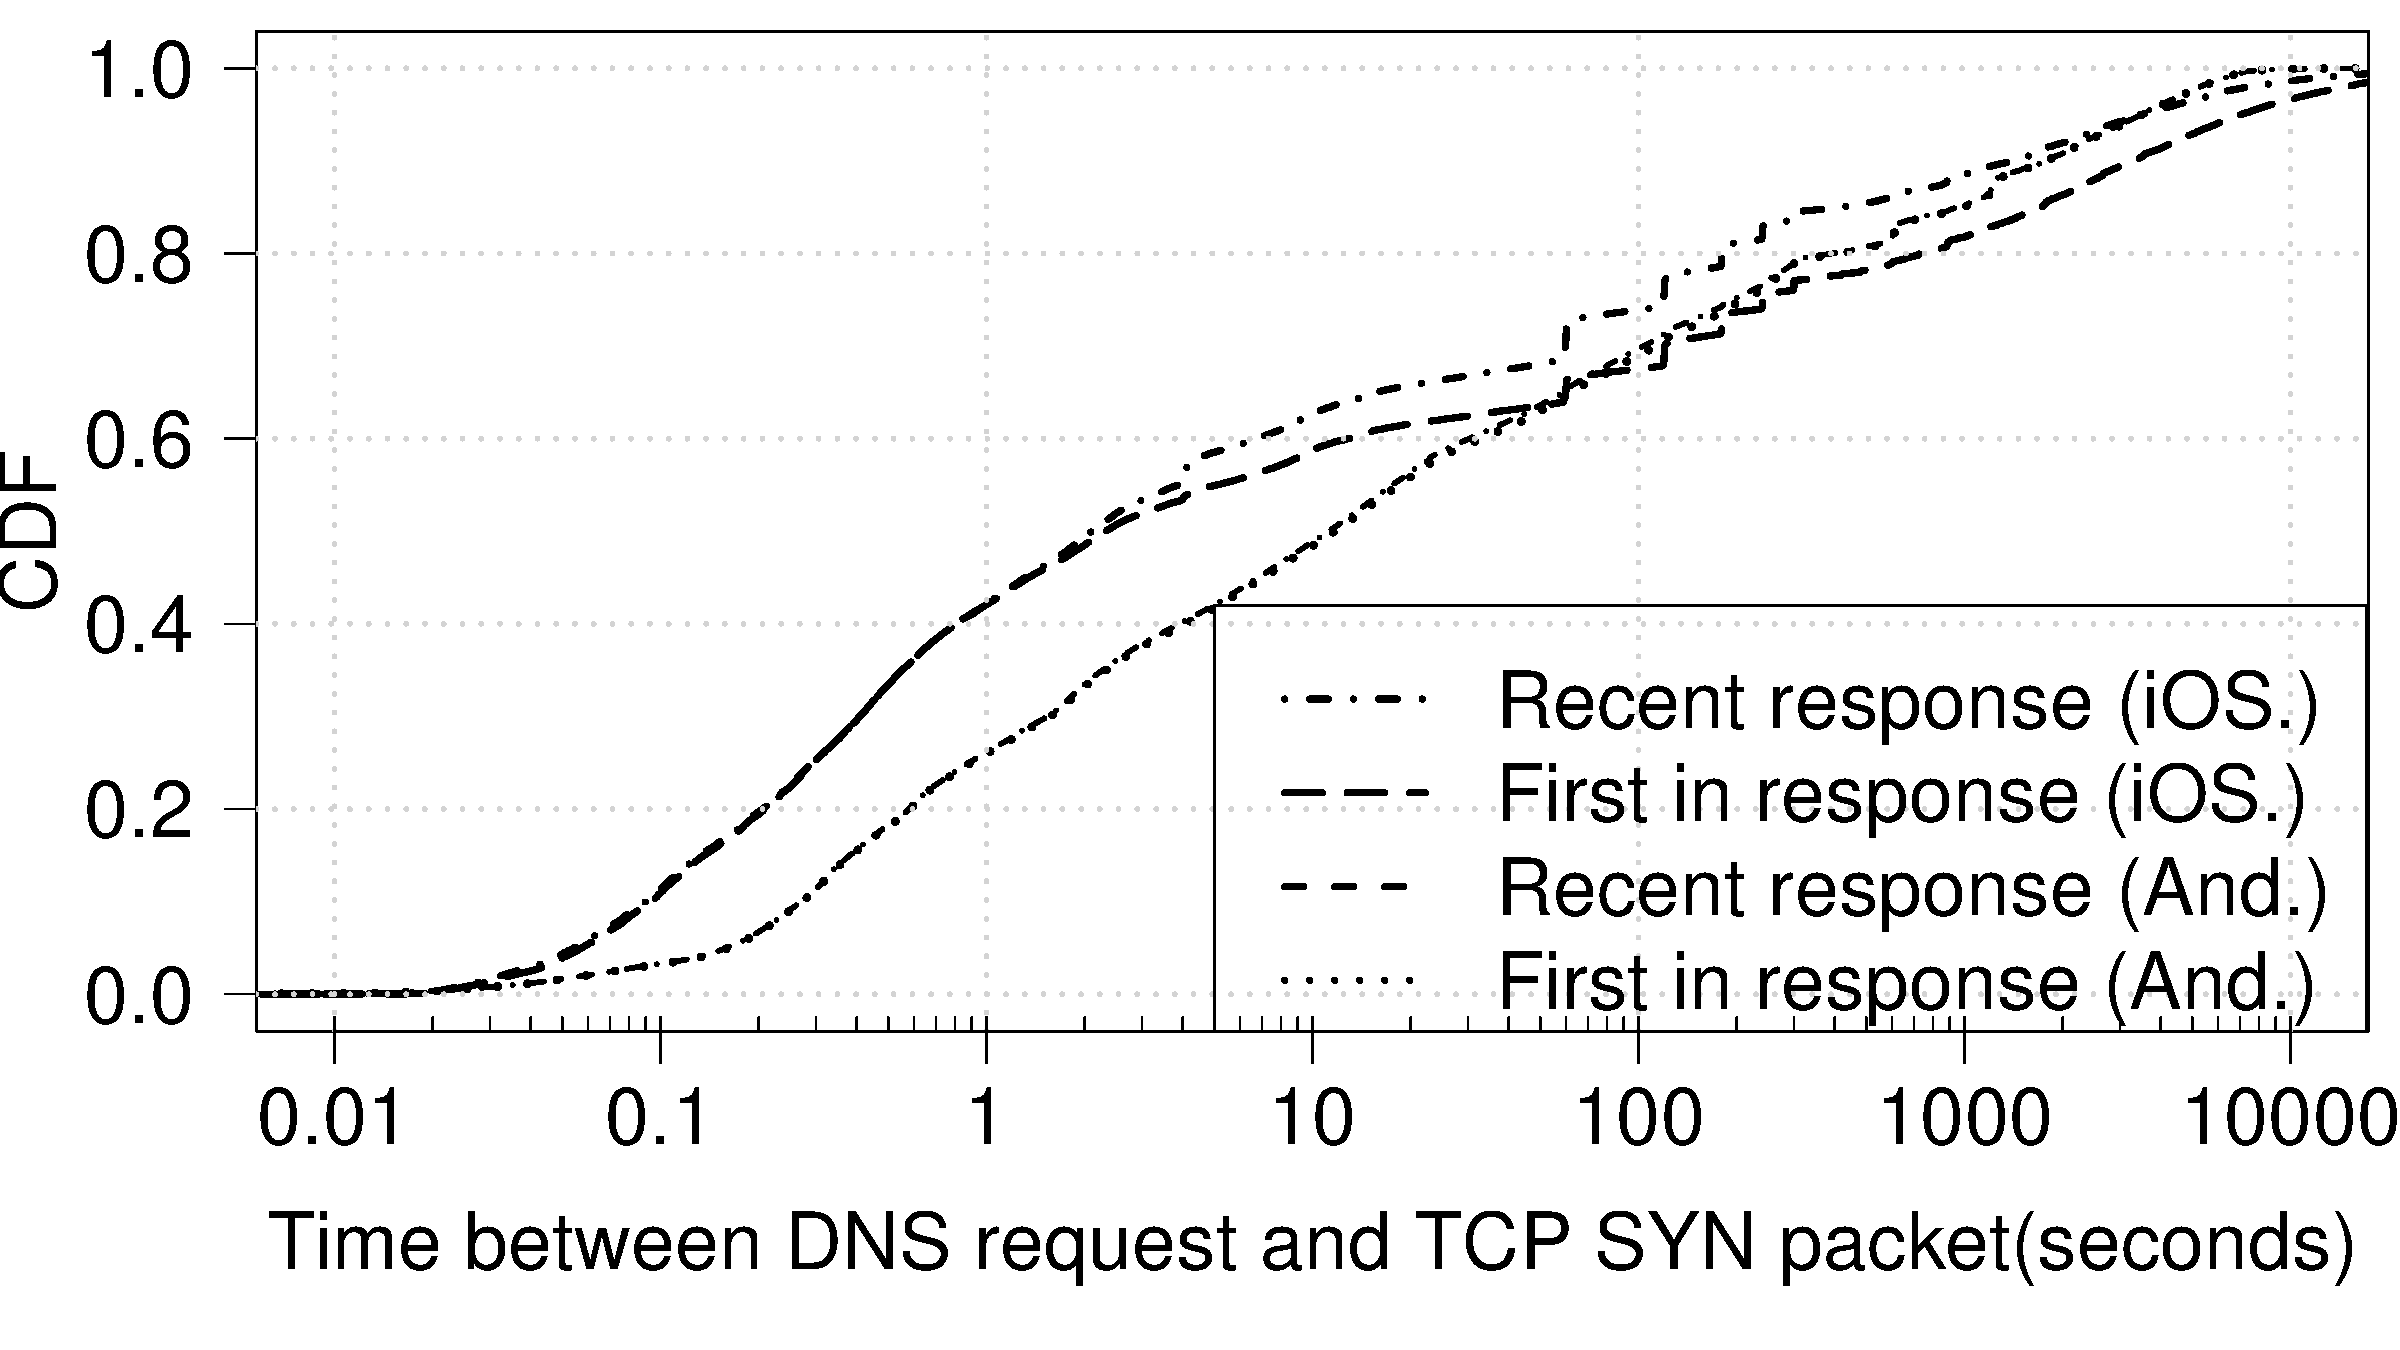
\includegraphics[width=\columnwidth]{plots/sslanalysis_dns_timediff_distrib.pdf}
% \caption{Distribution of the time between DNS response that contained the IP address of the SSL server and the SYN from the SSL flows. 
% \emph{The lack of difference in the curves for Android devices implies that the first entry in the most recent DNS response contained the IP address of the SSL flow.\tbd{rename xlab to DNS response.}}}
% \label{fig:ssl-dns-first-recent-distrib}
% \end{figure}

% To analyze the impact of the ambiguity, in \fref{fig:ssl-dns-first-recent-distrib} we plot the distribution of the time between the DNS response that contained the IP address and SYN packet from the SSL flow. 
% For this plot, we consider two types of DNS responses: the most recent DNS response that contain the IP address in the SSL flows, and the most recent DNS response that contained the IP address as the first entry in the DNS response. 
% We observe that for Android flows we do not observe a difference in the curves for the distribution, implying that the first entry in the most recent DNS response contained the IP address of the SSL flow.
% However, for iOS devices we observe a difference in the distribution when the time difference between the SYN and DNS response is larger than three seconds. 
% This difference creates an ambiguity which can be aggravated by caching of name resolution by the applications. 

We use the DNS flows that passed through \platname to further classify the SSL flows, a technique similar to DN-Hunter~\cite{bermudez:dnhunter}.
DN-Hunter relies on the most recent FQDN that corresponds to the IP address, however in our controlled experiments we observe Android and iOS devices prefer the the first entry in DNS response while resolving \emph{hostnames}.
Popular webservices such as google are known to use the same pool of IP addresses for various applications, for example the IP for gmail may also be used for search. 
In \fref{fig:ssl-classification-app-service} we present the fraction of SSL traffic where the most recent DNS response contained the IP address of the SSL flow in the first position. 
We observe that for the majority of SSL traffic by volume and flows can be classified by using the DNS responses. 

In summary, we use \platname to perform controlled experiments and in the wild measurements to characterize mobile Internet traffic. 
We use Bro to analyze the data and build on the output of bro to further classify HTTP flows and SSL flows to identify the source of the traffic. 
We now present the results of our experiments and measurements study. 


%%% Local Variables: 
%%% mode: latex
%%% TeX-master: "main"
%%% End: 


\section{Application Characterization}
\label{sec:characterize-app}

  We now turn to measurements of specific popular iOS and Android applications. 
  When users install apps, they grant them Internet access without detailed knowledge of how that access will be used, including {\it how much} data is sent or accessed, {\it what} data is sent,  or {\it with whom} the app communications.
  ``How much'' is important to conserve both bandwidth caps and battery capacity: an app which consumes or produces too much data will waste bandwidth resources, while an app which consumes or produces data too frequently will prevent the device radio from going idle to save power.
  ``With whom'' is important to protect users from excessive tracking -- the more organization's servers an app connects to, the more organizations which are able to track user behavior, location, or other private data.
  Finally, ``what data'' is important because apps may unnecessarily leak personally identifiable information (PII) such as user email address, IMEI, contact information, or other stored data either to the app provider or worse, to any eavesdropper on a public WiFi connection.
  We  report on our findings in all three of these dimensions for the iPhone and Android apps in our study.

\subsection{Bandwidth and Radio Usage}

  {\bf In the Wild.}
    \begin{itemize}
      \item Stats on how much bandwidth each user used; time of day; how frequent...
    \end{itemize}

  {\bf Android Apps.}
    To dig in to the root cause of these usage patterns, we also did an `app-by-app` analysis of network usage to see if most bandwidth consumption/radio time was the result of a few heavy applications, with most applications relatively idle, or whether usage was divided amongst all applications equally.
    In Figure~\ref{fig:app-by-app-usage}, we plot the CDF of total bytes transferred by each app in our study, one line for the top-100 Google Play apps we tested manually, and another for the top 2000 apps, tested automatically, from a third-party market.
    We see that...\tbd{Amy...}
    Regarding radio usage,...\tbd{Do we even have time to do this? I don't remember the exact metrics we used for the MobiSys submission.}

  {\bf iPhone Apps.}

\subsection{Third Party Servers}
  Many free applications support themselves financially by serving ads or providing resources for third parties to track user behavior.
  We now explore how many servers are contacted by a given app (\ie{} how many providers are tracking a user with this app) -- most of these typically for ads, tracking, or analytics -- as well as how much data is transferred to and from these servers (\ie{} how much does this traffic impact the user's data cap?).

  {\bf In the Wild.}
  We first consider the overall impact of these ads, analytic, and tracking services on typical user behavior in our IRB study...
  \tbd{Ashwin...}

\begin{figure}
\includegraphics[width=\columnwidth]{plots/ad_share_bytes.pdf}
\caption{Fraction of traffic volume because of Ads and Analytics. \emph{\tbd{Check for id1 and id25}}}
\label{fig:description}
\end{figure}

\begin{figure}
\includegraphics[width=\columnwidth]{plots/distrib_ad_uploads.pdf}
\caption{Distribution of bytes uploaded by ads and analytics sites. \emph{The distribution of bytes uploaded by all ads and analytics sites and the top four ads sites based on traffic volume across all users}.}
\label{fig:description}
\end{figure}

\begin{table}
\begin{small}
\begin{tabular}{|p{0.35\columnwidth}|p{0.1\columnwidth}|p{0.15\columnwidth}|p{0.1\columnwidth}|}
\hline
\multirow{2}{*}{\bf Tracker} & \multicolumn{3}{c|}{\bf Number of devices tracked}\tabularnewline
\cline{2-4}
   &  {\bf Total} & {\bf Android} & {\bf iOS} \tabularnewline
\hline
doubleclick.net & 25 & 11 & 14 \tabularnewline
\hline
google-analytics.com   & 25 & 11 & 14 \tabularnewline
\hline
googlesyndication.com  & 22 & 10 & 12 \tabularnewline
\hline
admob.com  & 21 & 10 & 11 \tabularnewline
\hline
scorecardresearch.com &  21 & 10 & 11 \tabularnewline
\hline
2mdn.net  &  20 & 9 &  11 \tabularnewline
\hline
atdmt.com  & 18 & 9 &  9 \tabularnewline
\hline
imrworldwide.com & 18 &  9 &  9 \tabularnewline
\hline
flurry.com & 17 & 7 &  10 \tabularnewline
\hline
googleadservices.com  & 17 & 8 &  9 \tabularnewline
\hline
\end{tabular}
\end{small}
\caption{The top 10 ads and analytics sites that tracked the devices in our dataset.
\emph{Two trackers, \emph{doubleclick.net} and\emph{google-analytics.com}, were tracking all the 25 devices in our dataset.}}
\label{tab:top_trackers}
\end{table}
\begin{figure}
\includegraphics[width=\columnwidth]{plots/num_uploading_trackers.pdf}
\caption{Distribution of bytes uploaded by ads and analytics sites. \emph{The distribution of bytes uploaded by all ads and analytics sites and the top four ads sites based on traffic volume across all users}.}
\label{fig:description}
\end{figure}


  {\bf Android Apps.}
  When we inspect the data from our controlled study, we see that some apps contact a large number of external servers while others contact significantly fewer.
  In Figure~\ref{fig:android-cdns}, we show both the total number of servers contacted (solid lines) as well as the number of organizations contacted (dotted lines) for both the top-100 Google Play dataset and the top-2000 third-party dataset.
  To quantify ``organizations contacted'', we performed whois lookups on all servers contacted and mapped them to an organization name, allowing us to tighten our upper bound on the number of companies/entities able to track the user through a single app.
  Returning to the figure, we see...~\ref{fig:android-cdns}...\tbd{Amy...}


  {\bf iPhone Apps.}
  \tbd{Shen...}

\subsection{Personally Identifiable Information}
  \begin{table*}
    \begin{tabular}{l|l|l|l|l|l|l|l|l|l}
       Dataset&Platform&\# Apps&Email&Location&Username&Password&Android ID&Contacts&IMEI\\
       \hline
       Google Play&Android&100&?&10 (10\%)&7 (7\%)&1 (1\%)&21 (21\%)&0 (0\%)&13 (13\%)\\
       \hline
       Third Party&Android&908&?&32 (3.5\%)&?&0 (0\%)&95 (10.4\%)&4 (0.4\%)&48 (5.3\%)\\
       \hline
       App Store&iPhone&100&?&?&?&?&?&?&?\\
    \end{tabular}
    \caption{Summary of personally identifiable information leaked in plaintext (HTTP) by Android and iPhone apps.}
  \end{table*}
  
  Finally, we turn to information leaked by individual applications. We do not report on data leaked for our real users here, but only the data leaked by our controlled apps in isolation.
  We consider data to be `leaked' when any personally identifiable information -- email address, phone number, IMEI number -- is sent across the network under HTTP or HTTPS.
  Naturally, some of this information may be relevant to the app -- most apps legitimately require email access. 
  However, none of this information should ever travel across the network in plaintext (HTTP), which we unfortunately see violated in serveral cases.

  To generate this data, we created fake user accounts on the test phones for a fake user named ``Tess Droid'', with fake contact information and fake Twitter and Facebook accounts. We were then able to check that none of this data ever was released over the network in plaintext.

  {\bf Android Apps.}
  Table 1 shows...

  {\bf iPhone Apps.}

%\subsection{Characterize Facebook Applications}

%Why Facebook was chosen?

%What do we observe ?

%What do we see in the User Agent Fields. 




\section{Application: \\
Revealing ISP Behavior}

This section describes how we build two applications atop \meddle to 
reveal the policies ISPs apply to mobile traffic traversing their networks. 
Previous work focused on addressing this problem in fixed-line networks; to 
the best of our knowledge we are the first to provide this functionality for 
mobile systems.

\subsection{Web Tripnets: Detecting ISP Content Manipulation}

ISPs, middleboxes and client software are known to change Web page content for 
a variety of reasons including performance optimization and security. In some cases, 
a third party can change a page for selfish reasons, \eg to insert ads that generate revenue 
for that party. Figure~\ref{fig:tripnet-example} depicts an example of content injection in China, where 
a banner ad is replaced by information about the local airport.

\begin{figure}
\centering
\includegraphics[width=0.9\linewidth]{figures/injectioncrop.png}
\caption{Screen capture of content injection by a Chinese ISP in November, 2013. The 
highlighted region at the bottom should be an advertisement from a US company. }
\label{fig:tripnet-example}
\end{figure}


This problem of Web interference was first highlighted by Reis~\etal~\cite{reis:tripwires}. 
The authors demonstrated that although a small percent of users were affected by in-flight changes, those changes tend to introduce vulnerabilities including cross-site scripting (XSS) attacks~\cite{reis:tripwires}. 
They proposed and deployed \emph{Web Tripwires}, a Javascript code to detect in-flight page changes. 
The main limitation of \emph{Web Tripwires} is that it requires each Web site to modify their content to include a tripwire.

In \meddle, we extended tripwires to alleviate this limitation. 
Namely, we use the HTTP proxy present in \meddle to inject a tripwire on \emph{any} page 
without requiring support from Web site developers -- an approach we call a \emph{Web Tripnet}.

\noindent\textbf{Implementation.} With \meddle all traffic is tunneled, thereby 
preventing ISPs from modifying pages. To help inform non-users of ISP content 
manipulation, we provide the Tripnet as an opt-in feature. Because this entails 
two fetches of every Web page, we also support two modes: always-on and low-rate random trials, where we 
insert tripwires for some small fraction of their visited sites.

The Tripnet works as follows (Fig.~\ref{fig:tripnet}. A client requests a Web page through the \meddle VPN 
tunnel. This request is forwarded to the destination server. The response returns to 
the \meddle server, where a transparent proxy injects the tripwire code.\footnote{We 
recognize the irony of injecting content to detect content injection, but this is done only with user consent.}
The tripwire-enabled response is forwarded to the client, which execute the javascript at page load time.


\begin{figure}
\centering
\includegraphics[width=0.9\linewidth]{figures/tripnet.pdf}
\caption{Overview of the \meddle Web-tripnet. A Web page is loaded
through the VPN tunnel, where a meddlebox inserts a Web tripwire. The
tripwire causes the browser to reload the Web page using the address of a
transparent proxy server that is accessed using an unencrypted connection.
After the proxied version of the page is loaded, the browser or a meddlebox
can compare the two pages to identify potential interference. }
\label{fig:tripnet}
\end{figure}

The tripwire code contains information about the page content prior to traversing the ISP. When 
executed, the code fetches the page again to compare with the (known) unmodified page content.  
To ensure that this fetch does \emph{not} traverse the VPN connection, we use a \emph{pigeonhole} domain 
whose traffic traverses an untunneled interface. For example, if the original request was for www.facebook.com, 
we send the request to tripnet.meddle.mobi/www.facebook.com/, where we run a Web proxy. 

When the request arrives at our proxy server, we could forward the request to the original target. In 
practice, however, doing so would return different content due to the highly dynamic nature of most 
Web content. Instead, we cache Web pages at the tripnet-injecting server and co-locate our Web proxy 
there. Thus we return exactly the same Web page that was received over the tunneled connection. 
Any difference in page content can only be due to ISP behavior. 


\noindent\textbf{Sites and ISPs tested.} We conducted controlled experiments using our Tripnet 
architecture, using the top 100 Web sites according to Alexa. We tested using 
AT\&T, T-Mobile and Verizon in the US, and Orange, Sosh and Bouygues in France. 
Many sites customize content according to User-Agent strings, so we spoof User-Agents 
as coming from iOS, Andriod and desktop clients.

\noindent\textbf{Page modification/injection.} Cases of manipulation of text content.

\noindent\textbf{Content modification.} In addition to detecting changes to text content in 
Web pages, we also use our controlled experiments to investigate whether ISPs are manipulating 
media content, \eg downsampling high-resolution images to reduce bandwidth consumption 
from mobile devices. For this experiment, we augment our Tripnet experiments with the result 
of wget results from the mobile device and the proxy server. Note that this experiment requires an 
app or tethered laptop to collect the Web media objects fetched over the mobile network.

Our results are as follows.

\noindent\textbf{Implications.} 


\subsection{App-Agnostic Replay: Detecting Service Differentiation}

Overview of the approach and challenges. \meddle allows us to capture 
traces from mobile devices over both \wifi and cell, meaning we can model 
behavior from either medium. \meddle also serves as a convenient location 
to conduct replay experiments. The challenge is how to capture and replay 
the salient features of application traffic such that it will be subject to differentiation 
from middleboxes. State what we can reproduce (timings, sequence of bytes, ports and source IPs) 
and what we cannot (destination IPs from client). Challenges with UDP. Challenges 
with different network conditions. Differences from Glasnost.

\textbf{Graph}: If we find a case of difference between \wifi and cell, plot it here.

Assumptions: ISPs will differentiate traffic based on hostname, IP addresses, ports, total number of 
connections, payload signatures, total bandwidth, time of day, ... \tbd{anything else?}

\noindent\textbf{Approach and feasibility.}
Description of adopted replay approach and tests to show validity.

\textbf{Graph}: Similarity score for network traffic in setting where we know there is no differentiation. 
Score can include overall throughput, latency characteristics, loss, packet timings.

\noindent\textbf{Wide-area testing.} Networks tested, observed behavior.

\textbf{Table}: each row is an app, each column is an ISP, each cell is a marker indicating what kind of 
differentiation is happening

\textbf{Graph}: Plot showing a sequence of traces that demonstrates what this differentiation looks like



\noindent\textbf{Content modification.} Downsampling, e.g.

\noindent\textbf{Implications.} 

\section{Application: Mobile Malware \\
Detection and Blocking}
\label{sec:malware}

%\subsection{Mobile infection vectors}
%
%\textbf{Two-second approach}: Get list of drive-by downloads for mobile. Potential sources:
%- Websites that post this stuff
%- Tweets by fake accounts from Alan's twitter data\
%- Other?
%
%Make a script that causes a device to load those malicious URLs. Identify malicious behavior from there.
%
%\textbf{Table}: Types of malicious URLs and what they do. Rows are URL types, columns are types of behavior, cells are counts/percentages/checkmarks. 

%\subsection{Mobile malware network analysis}

In the fixed-line environment, malware is used for botnets, spam, data exfiltration, and sabotage, among other 
purposes. Despite a handful of studies in the mobile space, little research has focused on the \emph{network 
properties} of malware in the mobile environment. In this section, we use \meddle to investigate malware network 
behavior and develop new techniques for detecting and blocking malware activity based exclusively on network 
activity.

\mypara{Assumptions and methodology} We base our analysis on the likely incentives for malware authors, mainly 
that they distribute malware for profit. In this setting, we observe that malware \emph{must} communicate some information 
to a remote service for coordination (\eg C\&C), exfiltration (stealing personal information) or billing (contacting toll services). 
We can detect the first two cases if they use IP; we cannot detect circuit switched activity such as sending SMS or making 
phone calls.

Focusing on IP traffic, \meddle gives us two opportunities to detect and block malware activity. First, we can detect 
the app binary being downloaded via a hash and block that transfer if it is identified as malware. Second, we can use network 
behavioral analysis to identify malicious activity from apps that passed through our hash filters and successfully installed. 
In the following paragraphs we describe how existing hash registries fail to capture most confirmed malware, how to 
use network activity to identify and block malware and how to augment hash registries by automatically identifying the 
malicious app binary responsible for the activity -- thus inoculating other users from this malware. Importantly, 
this approach works at machine instead of human timescales, protecting infected users and preventing new infections 
within minutes, not days.

\mypara{Dataset} To understand malware network behavior, we use a 
dataset consisting of 111 confirmed malicious Android APKs gathered by the Andrubis project~\cite{andrubis} in September, 2013.  
Similar to the approach in \S\ref{sec:dataset-contr-exper}, we conduct controlled experiments by installing 
a malware app on a clean OS with dummy user data, interacting with it for \tbd{X} minutes and recording the 
network traces using \meddle. To compare with non-malicous apps, we use the dataset gathered in \S\ref{sec:dataset}.

The malware consists of 46 families ranging from backdoors to spyware.  99 (89\%) of the apps generated network 
traffic, of which 91\% generated HTTP traffic. Many of the remaining apps targeted earlier versions of the Android 
OS and thus did not work in our tests. Note that although our study focuses on Android malware, our approach 
is applicable to iOS and other mobile OSes because it relies only on the ability to monitor network traffic.

\mypara{Signature-based detection is insufficient} First, we determine whether existing malware hash registries 
contain signatures for the malicious APKs in our data. Even in MONTH (X months after the malware was identified 
by Andrubis), we find that only Y\% of the apps in our dataset were correctly identified. This motivates the need 
for behavioral analysis.

\mypara{Malware exhibits distinctive network behavior} 
Previous work in fixed-line environments~\cite{perdisci:malwaresig} use network behavioral analysis to identify malware 
from network flows. In particular, they rely on \useragent information and perform clustering on this to distinguish 
malware from non-malicious traffic. In our dataset, we find that ...

Of the 99 apps generating network traffic, we observe that \tbd{}\% 
exfiltrate PII. Unique identifiers such as IMEI, Android ID and MAC address are most commonly leaked, and 
we further find 9 apps leaking telephone numbers. 

\mypara{Effectiveness of behavioral filters}
TBD 

%\subsection{Unsolicited traffic}
%Presumably there is none, but probably worth looking at inbound unsolicited traffic from a 
%\meddle instance with no users compared to one with active users. Might find something interesting there.
%


\section{Related Work}
\label{sec:related}

Placeholder for the papers.
\cite{thiagarajan:mobbat}

\cite{balasubramanian:encon}

\cite{vallina-rod:ads}

\cite{falaki:mobileusage}


\section{Conclusion}
\label{sec:conclusion}

Placeholder

{\footnotesize \bibliographystyle{acm}
\bibliography{biblio}}

%\theendnotes
\end{document}

%%% Local Variables: 
%%% mode: latex
%%% TeX-master: "meddle-main"
%%% End: 





